\documentclass[]{book}
\usepackage{lmodern}
\usepackage{amssymb,amsmath}
\usepackage{ifxetex,ifluatex}
\usepackage{fixltx2e} % provides \textsubscript
\ifnum 0\ifxetex 1\fi\ifluatex 1\fi=0 % if pdftex
  \usepackage[T1]{fontenc}
  \usepackage[utf8]{inputenc}
\else % if luatex or xelatex
  \ifxetex
    \usepackage{mathspec}
  \else
    \usepackage{fontspec}
  \fi
  \defaultfontfeatures{Ligatures=TeX,Scale=MatchLowercase}
\fi
% use upquote if available, for straight quotes in verbatim environments
\IfFileExists{upquote.sty}{\usepackage{upquote}}{}
% use microtype if available
\IfFileExists{microtype.sty}{%
\usepackage{microtype}
\UseMicrotypeSet[protrusion]{basicmath} % disable protrusion for tt fonts
}{}
\usepackage[margin=1in]{geometry}
\usepackage{hyperref}
\PassOptionsToPackage{usenames,dvipsnames}{color} % color is loaded by hyperref
\hypersetup{unicode=true,
            pdftitle={A Quick Start Guide to Survey Research},
            pdfauthor={Liz Carey (and hopefully many others)},
            colorlinks=true,
            linkcolor=Maroon,
            citecolor=Blue,
            urlcolor=Blue,
            breaklinks=true}
\urlstyle{same}  % don't use monospace font for urls
\usepackage{natbib}
\bibliographystyle{apalike}
\usepackage{color}
\usepackage{fancyvrb}
\newcommand{\VerbBar}{|}
\newcommand{\VERB}{\Verb[commandchars=\\\{\}]}
\DefineVerbatimEnvironment{Highlighting}{Verbatim}{commandchars=\\\{\}}
% Add ',fontsize=\small' for more characters per line
\usepackage{framed}
\definecolor{shadecolor}{RGB}{248,248,248}
\newenvironment{Shaded}{\begin{snugshade}}{\end{snugshade}}
\newcommand{\KeywordTok}[1]{\textcolor[rgb]{0.13,0.29,0.53}{\textbf{#1}}}
\newcommand{\DataTypeTok}[1]{\textcolor[rgb]{0.13,0.29,0.53}{#1}}
\newcommand{\DecValTok}[1]{\textcolor[rgb]{0.00,0.00,0.81}{#1}}
\newcommand{\BaseNTok}[1]{\textcolor[rgb]{0.00,0.00,0.81}{#1}}
\newcommand{\FloatTok}[1]{\textcolor[rgb]{0.00,0.00,0.81}{#1}}
\newcommand{\ConstantTok}[1]{\textcolor[rgb]{0.00,0.00,0.00}{#1}}
\newcommand{\CharTok}[1]{\textcolor[rgb]{0.31,0.60,0.02}{#1}}
\newcommand{\SpecialCharTok}[1]{\textcolor[rgb]{0.00,0.00,0.00}{#1}}
\newcommand{\StringTok}[1]{\textcolor[rgb]{0.31,0.60,0.02}{#1}}
\newcommand{\VerbatimStringTok}[1]{\textcolor[rgb]{0.31,0.60,0.02}{#1}}
\newcommand{\SpecialStringTok}[1]{\textcolor[rgb]{0.31,0.60,0.02}{#1}}
\newcommand{\ImportTok}[1]{#1}
\newcommand{\CommentTok}[1]{\textcolor[rgb]{0.56,0.35,0.01}{\textit{#1}}}
\newcommand{\DocumentationTok}[1]{\textcolor[rgb]{0.56,0.35,0.01}{\textbf{\textit{#1}}}}
\newcommand{\AnnotationTok}[1]{\textcolor[rgb]{0.56,0.35,0.01}{\textbf{\textit{#1}}}}
\newcommand{\CommentVarTok}[1]{\textcolor[rgb]{0.56,0.35,0.01}{\textbf{\textit{#1}}}}
\newcommand{\OtherTok}[1]{\textcolor[rgb]{0.56,0.35,0.01}{#1}}
\newcommand{\FunctionTok}[1]{\textcolor[rgb]{0.00,0.00,0.00}{#1}}
\newcommand{\VariableTok}[1]{\textcolor[rgb]{0.00,0.00,0.00}{#1}}
\newcommand{\ControlFlowTok}[1]{\textcolor[rgb]{0.13,0.29,0.53}{\textbf{#1}}}
\newcommand{\OperatorTok}[1]{\textcolor[rgb]{0.81,0.36,0.00}{\textbf{#1}}}
\newcommand{\BuiltInTok}[1]{#1}
\newcommand{\ExtensionTok}[1]{#1}
\newcommand{\PreprocessorTok}[1]{\textcolor[rgb]{0.56,0.35,0.01}{\textit{#1}}}
\newcommand{\AttributeTok}[1]{\textcolor[rgb]{0.77,0.63,0.00}{#1}}
\newcommand{\RegionMarkerTok}[1]{#1}
\newcommand{\InformationTok}[1]{\textcolor[rgb]{0.56,0.35,0.01}{\textbf{\textit{#1}}}}
\newcommand{\WarningTok}[1]{\textcolor[rgb]{0.56,0.35,0.01}{\textbf{\textit{#1}}}}
\newcommand{\AlertTok}[1]{\textcolor[rgb]{0.94,0.16,0.16}{#1}}
\newcommand{\ErrorTok}[1]{\textcolor[rgb]{0.64,0.00,0.00}{\textbf{#1}}}
\newcommand{\NormalTok}[1]{#1}
\usepackage{longtable,booktabs}
\usepackage{graphicx,grffile}
\makeatletter
\def\maxwidth{\ifdim\Gin@nat@width>\linewidth\linewidth\else\Gin@nat@width\fi}
\def\maxheight{\ifdim\Gin@nat@height>\textheight\textheight\else\Gin@nat@height\fi}
\makeatother
% Scale images if necessary, so that they will not overflow the page
% margins by default, and it is still possible to overwrite the defaults
% using explicit options in \includegraphics[width, height, ...]{}
\setkeys{Gin}{width=\maxwidth,height=\maxheight,keepaspectratio}
\IfFileExists{parskip.sty}{%
\usepackage{parskip}
}{% else
\setlength{\parindent}{0pt}
\setlength{\parskip}{6pt plus 2pt minus 1pt}
}
\setlength{\emergencystretch}{3em}  % prevent overfull lines
\providecommand{\tightlist}{%
  \setlength{\itemsep}{0pt}\setlength{\parskip}{0pt}}
\setcounter{secnumdepth}{5}
% Redefines (sub)paragraphs to behave more like sections
\ifx\paragraph\undefined\else
\let\oldparagraph\paragraph
\renewcommand{\paragraph}[1]{\oldparagraph{#1}\mbox{}}
\fi
\ifx\subparagraph\undefined\else
\let\oldsubparagraph\subparagraph
\renewcommand{\subparagraph}[1]{\oldsubparagraph{#1}\mbox{}}
\fi

%%% Use protect on footnotes to avoid problems with footnotes in titles
\let\rmarkdownfootnote\footnote%
\def\footnote{\protect\rmarkdownfootnote}

%%% Change title format to be more compact
\usepackage{titling}

% Create subtitle command for use in maketitle
\newcommand{\subtitle}[1]{
  \posttitle{
    \begin{center}\large#1\end{center}
    }
}

\setlength{\droptitle}{-2em}
  \title{A Quick Start Guide to Survey Research}
  \pretitle{\vspace{\droptitle}\centering\huge}
  \posttitle{\par}
  \author{Liz Carey (and hopefully many others)}
  \preauthor{\centering\large\emph}
  \postauthor{\par}
  \predate{\centering\large\emph}
  \postdate{\par}
  \date{2019-01-07}

\usepackage{booktabs}

\begin{document}
\maketitle

{
\hypersetup{linkcolor=black}
\setcounter{tocdepth}{1}
\tableofcontents
}
\chapter*{Welcome to survey research}\label{welcome-to-survey-research}
\addcontentsline{toc}{chapter}{Welcome to survey research}

\begin{figure}
\centering

\includegraphics{figs/sponge_bob.png}
\caption{}
\end{figure}

This book is intended to be a quick resource for conducting survey
research. By no means is it intended to be comprehensive of all survey
research methodologies.

\chapter*{Preface}\label{preface}
\addcontentsline{toc}{chapter}{Preface}

It can be difficult to find condensed and easy to read resources on
survey research.

We developed this book in the hopes of future collaboration among other
UX researchers.

\section*{Outline}\label{outline}
\addcontentsline{toc}{section}{Outline}

The content of the book will include:

\begin{itemize}
\tightlist
\item
  \textbf{Chapter 1}
\item
  \textbf{Chapter 2}
\end{itemize}

\section*{Prerequisites}\label{prerequisites}
\addcontentsline{toc}{section}{Prerequisites}

All you need is an interest in conducting survey research, we'll assume
basic knowledge, and hope to include code snippets (python and R) along
the way

\section*{Acknowledgements}\label{acknowledgements}
\addcontentsline{toc}{section}{Acknowledgements}

This book wouldn't be possible without the contributions of:

\chapter{Designing a survey}\label{macro}

\section{What is your research goal?}\label{what-is-your-research-goal}

First, establish if a survey is the right method to accomplish your
research goal by asking yourself:

\begin{itemize}
\tightlist
\item
  What do you currently know?
\item
  What \emph{don't} you know?
\end{itemize}

Below is a useful visualization from the Nielsen Norman group on how to
decide between which qualitative or quantitative methods to answer your
research goal \citep{nng_method}.

\begin{center}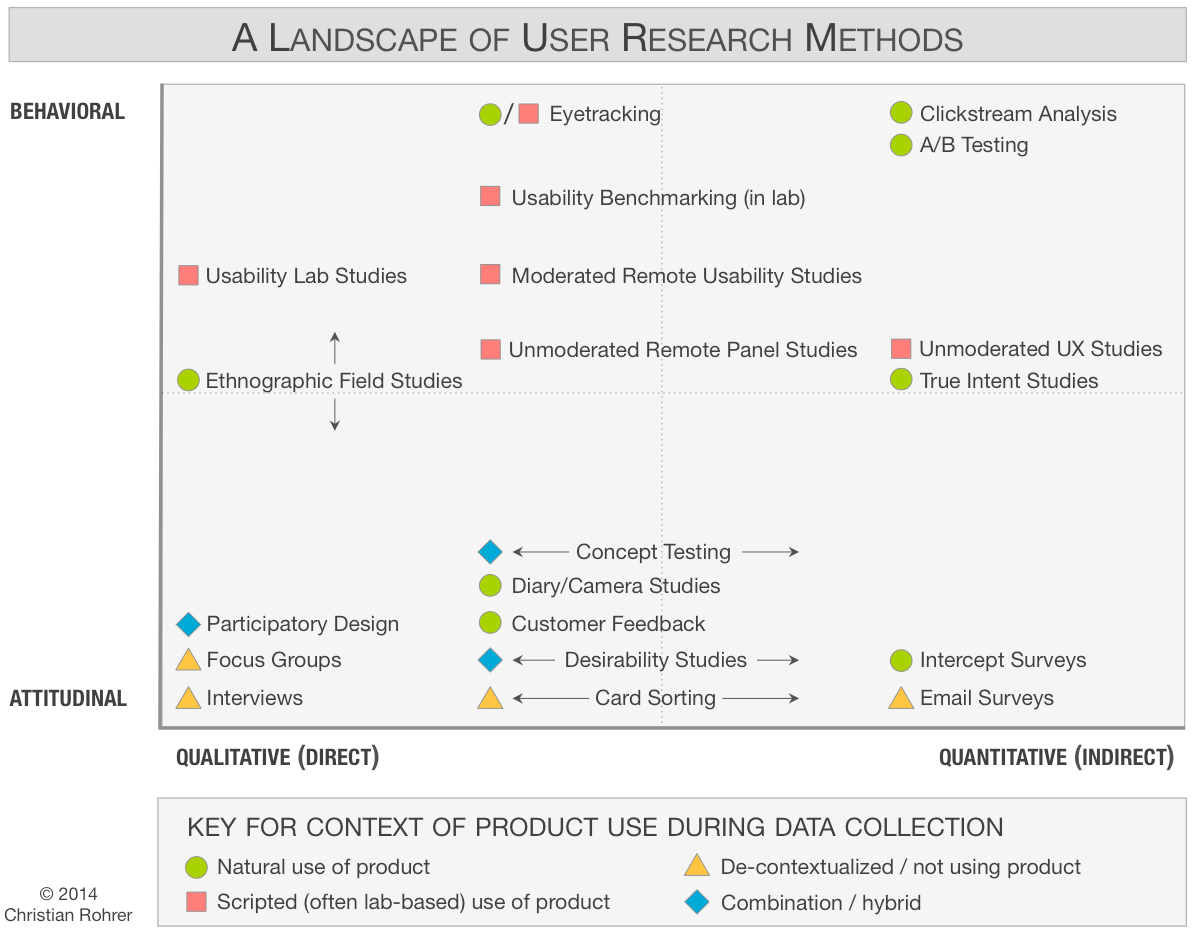
\includegraphics{figs/nng_ux_methods_chart2} \end{center}

Surveys are great for answering the ``How many and how much'' of what
people do and say; surveys are not the best method at understanding the
``Why and how to fix'' a product problem.

\begin{figure}
\centering
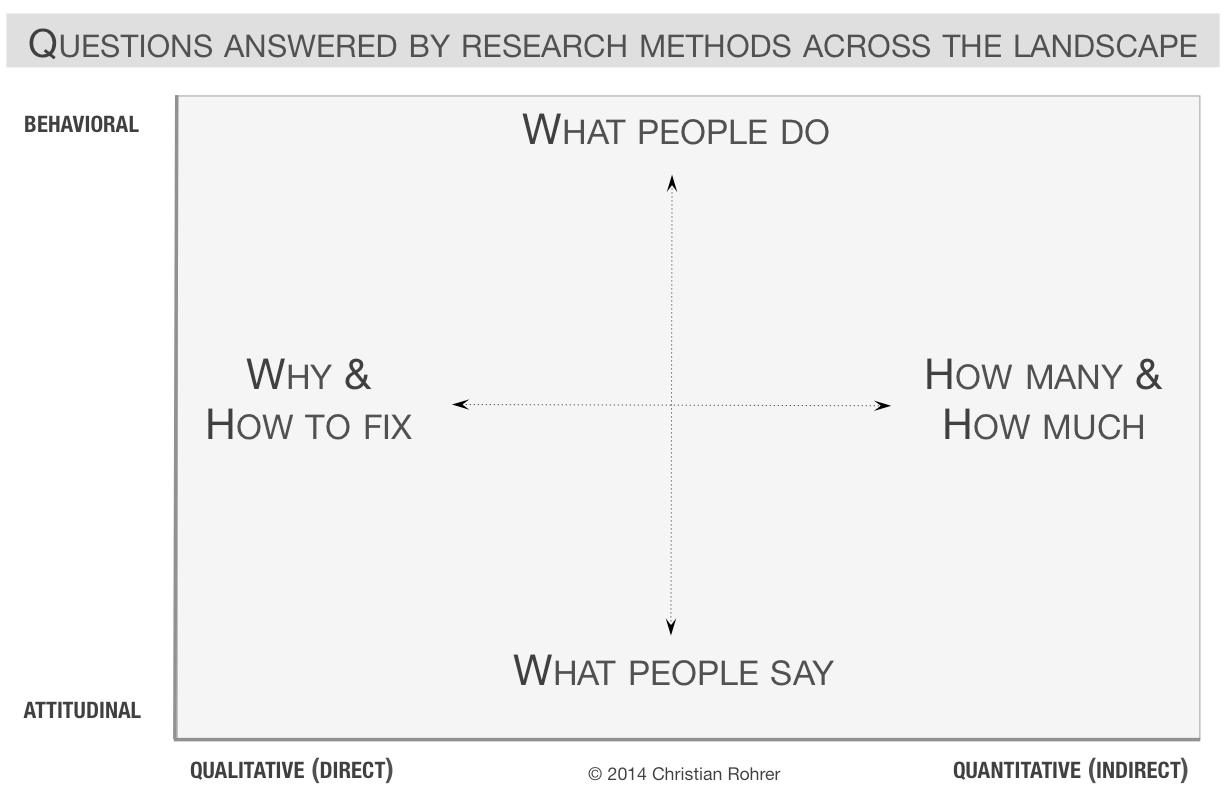
\includegraphics{figs/nng_ux_methods_chart.png}
\caption{}
\end{figure}

\section{Who are you studying?}\label{who-are-you-studying}

This question may be simple at first, but when you start to narrow down

\chapter{Writing effective survey
questions}\label{writing-effective-survey-questions}

Effective survey questions result in \textbf{consistent} and
\textbf{reliable} responses.

\chapter{Survey Analysis}\label{analysis}

After you've fielded your survey, here are the steps to making sense of
the data.

This section assumes you have a laptop set up to work with in either R
or python. Head over to the Appendix page if you need help with set up.

\section{Organize your workspace}\label{organize-your-workspace}

Before beginning any analysis, you'll want to set up a reproducible
workflow in your workspace. Below is an adapted suggestion on how to
organize your workspace from Ben Marwick, Carl Boettiger, and Lincoln
Mullen \citep{reproducible_workflow}

\begin{verbatim}
project
|- DESCRIPTION          # project metadata and dependencies 
|- README.md            # top-level description of content and guide to users
|
|- data/                # data files used 
|  +- raw_data.csv      # data files in open formats such as TXT, CSV, TSV, etc.
|  +- cleaned_data.csv  # data files that have been cleaned, merged, etc that you'll use for survey analysis
|
|- analysis/            # any programmatic code
|  +- my_report.Rmd     # R markdown file with narrative text interwoven with code chunks 
|  +- makefile          # builds a PDF/HTML/DOCX file from the Rmd, code, and data files
|  +- scripts/          # code files (R, shell, etc.) used for data cleaning, analysis and visualisation 
|
|- R/                     
|  +- my_functions.R    # custom R functions that are used more than once throughout the project
|
|- man/
|  +- my_functions.Rd   # documentation for the R functions (auto-generated when using devtools)
|
\end{verbatim}

\section{Data Cleaning}\label{data-cleaning}

Before you can begin looking at the results, you'll need to clean the
data.

\subsection{Load the data}\label{load-the-data}

Download your raw survey data as a csv and load it into your your
analysis tool of choice (e.g.~Ipython notebook or Rstudio)

\textbf{R version}

\begin{Shaded}
\begin{Highlighting}[]
\CommentTok{#load necessary packages for analysis}
\KeywordTok{library}\NormalTok{(tidyverse)}

\CommentTok{#read/store the data as the variable df (short for dataframe)}
\NormalTok{df <-}\StringTok{ }\KeywordTok{read_csv}\NormalTok{(file)}
\end{Highlighting}
\end{Shaded}

\textbf{python version}

\begin{Shaded}
\begin{Highlighting}[]
\CommentTok{#load necessary modules for analysis}
\NormalTok{import pandas as pd}

\CommentTok{#read/store the data as the variable df (short for dataframe)}
\NormalTok{df =}\StringTok{ }\KeywordTok{pd.read_csv}\NormalTok{(filename)}
\end{Highlighting}
\end{Shaded}

\subsection{Preview the data}\label{preview-the-data}

It's important to get a look at the data to spot an errors in uploading,
etc.

\appendix


\chapter{Setting up R}\label{appendixA}

\section{Package installation}\label{package-installation}

You'll want to install the following packages:

\begin{Shaded}
\begin{Highlighting}[]
\KeywordTok{library}\NormalTok{(tidyverse)}
\end{Highlighting}
\end{Shaded}

\chapter{Setting up python}\label{appendixB}

\begin{Shaded}
\begin{Highlighting}[]
\CommentTok{# Pandas makes working with data tables easier}
\NormalTok{import pandas as pd}

\CommentTok{# Numpy is a library for working with Arrays}
\NormalTok{import numpy as np}

\CommentTok{# Module for plotting graphs}
\NormalTok{import matplotlib.pyplot as plt}
\NormalTok{import seaborn as sns}

\CommentTok{# SciPy implements many different numerical algorithms}
\NormalTok{import scipy.stats as stats}
\NormalTok{import collections}
\end{Highlighting}
\end{Shaded}

\begin{Shaded}
\begin{Highlighting}[]
\KeywordTok{library}\NormalTok{(tidyverse)}
\end{Highlighting}
\end{Shaded}

\bibliography{book.bib,packages.bib}


\end{document}
